%%%%%%%%%%%%%%%%%%%%%%%%%%%%%%%%%%%%%%%%%
% Quality Report Format 
% Derived from The Legrand Orange Book LaTeX Template (Overleaf)
%%%%%%%%%%%%%%%%%%%%%%%%%%%%%%%%%%%%%%%%%

% May be able to just run LaTex -> PDF (Latexmk) in LaTexilla

%Otherwise,
% When you first open the template, compile it from the command line with the 
% commands below to make sure your LaTeX distribution is configured correctly:
% Re-run to get TOC
% 1) pdflatex Retaining_Volunteers_20171103
% 2) biber Retaining_Volunteers_20171103
% 3) pdflatex Retaining_Volunteers_20171103 x 2

% run LaTex -> PDF (Latexmk) in LaTexilla to get .idx file
% then
% 1) pdflatex Retaining_Volunteers_20171103
% 2) makeindex Retaining_Volunteers_20171103.idx -s StyleInd.ist
% 3) biber Retaining_Volunteers_20171103
% 4) pdflatex Retaining_Volunteers_20171103 x 2
% 

%%%%%%%%%%%%%%%%%%%%%%%%%%%%%%%%
%GRAPHICS
%%%%%%%%%%%%%%%%%%%%%%%%%%%%%%%%%
% graphics for cover photo and chapter photos must be .jpeg



%----------------------------------------------------------------------------------------
%	PACKAGES AND OTHER DOCUMENT CONFIGURATIONS
%----------------------------------------------------------------------------------------

\documentclass[11pt,fleqn]{book} % Default font size and left-justified equations

%----------------------------------------------------------------------------------------
%	VARIOUS REQUIRED PACKAGES
%----------------------------------------------------------------------------------------

\usepackage{titlesec} % Allows customization of titles

\usepackage{graphicx} % Required for including pictures
\graphicspath{{Pictures/}} % Specifies the directory where pictures are stored

\usepackage{lipsum} % Inserts dummy text

\usepackage{tikz} % Required for drawing custom shapes

\usepackage[american]{babel} % English language/hyphenation

\usepackage{enumitem} % Customize lists
\setlist{nolistsep} % Reduce spacing between bullet points and numbered lists

\usepackage{booktabs} % Required for nicer horizontal rules in tables

\usepackage{eso-pic} % Required for specifying an image background in the title page

%----------------------------------------------------------------------------------------
%	MAIN TABLE OF CONTENTS
%----------------------------------------------------------------------------------------

\usepackage{titletoc} % Required for manipulating the table of contents

\contentsmargin{0cm} % Removes the default margin
% Chapter text styling
\titlecontents{chapter}[1.25cm] % Indentation
{\addvspace{15pt}\large\sffamily\bfseries} % Spacing and font options for chapters
{\color{ocre!60}\contentslabel[\Large\thecontentslabel]{1.25cm}\color{ocre}} % Chapter number
{}  
{\color{ocre!60}\normalsize\sffamily\bfseries\;\titlerule*[.5pc]{.}\;\thecontentspage} % Page number
% Section text styling
\titlecontents{section}[1.25cm] % Indentation
{\addvspace{5pt}\sffamily\bfseries} % Spacing and font options for sections
{\contentslabel[\thecontentslabel]{1.25cm}} % Section number
{}
{\sffamily\hfill\color{black}\thecontentspage} % Page number
[]
% Subsection text styling
\titlecontents{subsection}[1.25cm] % Indentation
{\addvspace{1pt}\sffamily\small} % Spacing and font options for subsections
{\contentslabel[\thecontentslabel]{1.25cm}} % Subsection number
{}
{\sffamily\;\titlerule*[.5pc]{.}\;\thecontentspage} % Page number
[] 

%----------------------------------------------------------------------------------------
%	MINI TABLE OF CONTENTS IN CHAPTER HEADS
%----------------------------------------------------------------------------------------

% Section text styling
\titlecontents{lsection}[0em] % Indendating
{\footnotesize\sffamily} % Font settings
{}
{}
{}

% Subsection text styling
\titlecontents{lsubsection}[.5em] % Indentation
{\normalfont\footnotesize\sffamily} % Font settings
{}
{}
{}
 
%----------------------------------------------------------------------------------------
%	PAGE HEADERS
%----------------------------------------------------------------------------------------

\usepackage{fancyhdr} % Required for header and footer configuration

\pagestyle{fancy}
\renewcommand{\chaptermark}[1]{\markboth{\sffamily\normalsize\bfseries\chaptername\ \thechapter.\ #1}{}} % Chapter text font settings
\renewcommand{\sectionmark}[1]{\markright{\sffamily\normalsize\thesection\hspace{5pt}#1}{}} % Section text font settings
\fancyhf{} \fancyhead[LE,RO]{\sffamily\normalsize\thepage} % Font setting for the page number in the header
\fancyhead[LO]{\rightmark} % Print the nearest section name on the left side of odd pages
\fancyhead[RE]{\leftmark} % Print the current chapter name on the right side of even pages
\renewcommand{\headrulewidth}{0.5pt} % Width of the rule under the header
\addtolength{\headheight}{2.5pt} % Increase the spacing around the header slightly
\renewcommand{\footrulewidth}{0pt} % Removes the rule in the footer
\fancypagestyle{plain}{\fancyhead{}\renewcommand{\headrulewidth}{0pt}} % Style for when a plain pagestyle is specified

% Removes the header from odd empty pages at the end of chapters
\makeatletter
\renewcommand{\cleardoublepage}{
\clearpage\ifodd\c@page\else
\hbox{}
\vspace*{\fill}
\thispagestyle{empty}
\newpage
\fi}

%----------------------------------------------------------------------------------------
%	THEOREM STYLES
%----------------------------------------------------------------------------------------

\usepackage{amsmath,amsfonts,amssymb,amsthm} % For math equations, theorems, symbols, etc

\newcommand{\intoo}[2]{\mathopen{]}#1\,;#2\mathclose{[}}
\newcommand{\ud}{\mathop{\mathrm{{}d}}\mathopen{}}
\newcommand{\intff}[2]{\mathopen{[}#1\,;#2\mathclose{]}}
\newtheorem{notation}{Notation}[chapter]

%%%%%%%%%%%%%%%%%%%%%%%%%%%%%%%%%%%%%%%%%%%%%%%%%%%%%%%%%%%%%%%%%%%%%%%%%%%
%%%%%%%%%%%%%%%%%%%% dedicated to boxed/framed environements %%%%%%%%%%%%%%
%%%%%%%%%%%%%%%%%%%%%%%%%%%%%%%%%%%%%%%%%%%%%%%%%%%%%%%%%%%%%%%%%%%%%%%%%%%
\newtheoremstyle{ocrenumbox}% % Theorem style name
{0pt}% Space above
{0pt}% Space below
{\normalfont}% % Body font
{}% Indent amount
{\small\bf\sffamily\color{ocre}}% % Theorem head font
{\;}% Punctuation after theorem head
{0.25em}% Space after theorem head
{\small\sffamily\color{ocre}\thmname{#1}\nobreakspace\thmnumber{\@ifnotempty{#1}{}\@upn{#2}}% Theorem text (e.g. Theorem 2.1)
\thmnote{\nobreakspace\the\thm@notefont\sffamily\bfseries\color{black}---\nobreakspace#3.}} % Optional theorem note
\renewcommand{\qedsymbol}{$\blacksquare$}% Optional qed square

\newtheoremstyle{blacknumex}% Theorem style name
{5pt}% Space above
{5pt}% Space below
{\normalfont}% Body font
{} % Indent amount
{\small\bf\sffamily}% Theorem head font
{\;}% Punctuation after theorem head
{0.25em}% Space after theorem head
{\small\sffamily{\tiny\ensuremath{\blacksquare}}\nobreakspace\thmname{#1}\nobreakspace\thmnumber{\@ifnotempty{#1}{}\@upn{#2}}% Theorem text (e.g. Theorem 2.1)
\thmnote{\nobreakspace\the\thm@notefont\sffamily\bfseries---\nobreakspace#3.}}% Optional theorem note

\newtheoremstyle{blacknumbox} % Theorem style name
{0pt}% Space above
{0pt}% Space below
{\normalfont}% Body font
{}% Indent amount
{\small\bf\sffamily}% Theorem head font
{\;}% Punctuation after theorem head
{0.25em}% Space after theorem head
{\small\sffamily\thmname{#1}\nobreakspace\thmnumber{\@ifnotempty{#1}{}\@upn{#2}}% Theorem text (e.g. Theorem 2.1)
\thmnote{\nobreakspace\the\thm@notefont\sffamily\bfseries---\nobreakspace#3.}}% Optional theorem note

%%%%%%%%%%%%%%%%%%%%%%%%%%%%%%%%%%%%%%%%%%%%%%%%%%%%%%%%%%%%%%%%%%%%%%%%%%%
%%%%%%%%%%%%% dedicated to non-boxed/non-framed environements %%%%%%%%%%%%%
%%%%%%%%%%%%%%%%%%%%%%%%%%%%%%%%%%%%%%%%%%%%%%%%%%%%%%%%%%%%%%%%%%%%%%%%%%%
\newtheoremstyle{ocrenum}% % Theorem style name
{5pt}% Space above
{5pt}% Space below
{\normalfont}% % Body font
{}% Indent amount
{\small\bf\sffamily\color{ocre}}% % Theorem head font
{\;}% Punctuation after theorem head
{0.25em}% Space after theorem head
{\small\sffamily\color{ocre}\thmname{#1}\nobreakspace\thmnumber{\@ifnotempty{#1}{}\@upn{#2}}% Theorem text (e.g. Theorem 2.1)
\thmnote{\nobreakspace\the\thm@notefont\sffamily\bfseries\color{black}---\nobreakspace#3.}} % Optional theorem note
\renewcommand{\qedsymbol}{$\blacksquare$}% Optional qed square
\makeatother

% Defines the theorem text style for each type of theorem to one of the three styles above
\newcounter{dummy} 
\numberwithin{dummy}{section}
\theoremstyle{ocrenumbox}
\newtheorem{theoremeT}[dummy]{Theorem}
\newtheorem{problem}{Problem}[chapter]
\newtheorem{exerciseT}{Exercise}[chapter]
\theoremstyle{blacknumex}
\newtheorem{exampleT}{Example}[chapter]
\theoremstyle{blacknumbox}
\newtheorem{vocabulary}{Vocabulary}[chapter]
\newtheorem{definitionT}{Definition}[section]
\newtheorem{corollaryT}[dummy]{Corollary}
\theoremstyle{ocrenum}
\newtheorem{proposition}[dummy]{Proposition}

%----------------------------------------------------------------------------------------
%	DEFINITION OF COLORED BOXES
%----------------------------------------------------------------------------------------

\RequirePackage[framemethod=default]{mdframed} % Required for creating the theorem, definition, exercise and corollary boxes

% Theorem box
\newmdenv[skipabove=7pt,
skipbelow=7pt,
backgroundcolor=black!5,
linecolor=ocre,
innerleftmargin=5pt,
innerrightmargin=5pt,
innertopmargin=5pt,
leftmargin=0cm,
rightmargin=0cm,
innerbottommargin=5pt]{tBox}

% Exercise box	  
\newmdenv[skipabove=7pt,
skipbelow=7pt,
rightline=false,
leftline=true,
topline=false,
bottomline=false,
backgroundcolor=ocre!10,
linecolor=ocre,
innerleftmargin=5pt,
innerrightmargin=5pt,
innertopmargin=5pt,
innerbottommargin=5pt,
leftmargin=0cm,
rightmargin=0cm,
linewidth=4pt]{eBox}	

% Definition box
\newmdenv[skipabove=7pt,
skipbelow=7pt,
rightline=false,
leftline=true,
topline=false,
bottomline=false,
linecolor=ocre,
innerleftmargin=5pt,
innerrightmargin=5pt,
innertopmargin=0pt,
leftmargin=0cm,
rightmargin=0cm,
linewidth=4pt,
innerbottommargin=0pt]{dBox}	

% Corollary box
\newmdenv[skipabove=7pt,
skipbelow=7pt,
rightline=false,
leftline=true,
topline=false,
bottomline=false,
linecolor=gray,
backgroundcolor=black!5,
innerleftmargin=5pt,
innerrightmargin=5pt,
innertopmargin=5pt,
leftmargin=0cm,
rightmargin=0cm,
linewidth=4pt,
innerbottommargin=5pt]{cBox}

% Creates an environment for each type of theorem and assigns it a theorem text style from the "Theorem Styles" section above and a colored box from above
\newenvironment{theorem}{\begin{tBox}\begin{theoremeT}}{\end{theoremeT}\end{tBox}}
\newenvironment{exercise}{\begin{eBox}\begin{exerciseT}}{\hfill{\color{ocre}\tiny\ensuremath{\blacksquare}}\end{exerciseT}\end{eBox}}				  
\newenvironment{definition}{\begin{dBox}\begin{definitionT}}{\end{definitionT}\end{dBox}}	
\newenvironment{example}{\begin{exampleT}}{\hfill{\tiny\ensuremath{\blacksquare}}\end{exampleT}}		
\newenvironment{corollary}{\begin{cBox}\begin{corollaryT}}{\end{corollaryT}\end{cBox}}	

%----------------------------------------------------------------------------------------
%	REMARK ENVIRONMENT
%----------------------------------------------------------------------------------------

\newenvironment{remark}{\par\vspace{10pt}\small % Vertical white space above the remark and smaller font size
\begin{list}{}{
\leftmargin=35pt % Indentation on the left
\rightmargin=25pt}\item\ignorespaces % Indentation on the right
\makebox[-2.5pt]{\begin{tikzpicture}[overlay]
\node[draw=ocre!60,line width=1pt,circle,fill=ocre!25,font=\sffamily\bfseries,inner sep=2pt,outer sep=0pt] at (-15pt,0pt){\textcolor{ocre}{R}};\end{tikzpicture}} % Orange R in a circle
\advance\baselineskip -1pt}{\end{list}\vskip5pt} % Tighter line spacing and white space after remark

%----------------------------------------------------------------------------------------
%	SECTION NUMBERING IN THE MARGIN
%----------------------------------------------------------------------------------------

\makeatletter
\renewcommand{\@seccntformat}[1]{\llap{\textcolor{ocre}{\csname the#1\endcsname}\hspace{1em}}}                    
\renewcommand{\section}{\@startsection{section}{1}{\z@}
{-4ex \@plus -1ex \@minus -.4ex}
{1ex \@plus.2ex }
{\normalfont\large\sffamily\bfseries}}
\renewcommand{\subsection}{\@startsection {subsection}{2}{\z@}
{-3ex \@plus -0.1ex \@minus -.4ex}
{0.5ex \@plus.2ex }
{\normalfont\sffamily\bfseries}}
\renewcommand{\subsubsection}{\@startsection {subsubsection}{3}{\z@}
{-2ex \@plus -0.1ex \@minus -.2ex}
{.2ex \@plus.2ex }
{\normalfont\small\sffamily\bfseries}}                        
\renewcommand\paragraph{\@startsection{paragraph}{4}{\z@}
{-2ex \@plus-.2ex \@minus .2ex}
{.1ex}
{\normalfont\small\sffamily\bfseries}}

%----------------------------------------------------------------------------------------
%	HYPERLINKS IN THE DOCUMENTS
%----------------------------------------------------------------------------------------

% For an unclear reason, the package should be loaded now and not later
\usepackage{hyperref}
\hypersetup{hidelinks,backref=true,pagebackref=true,hyperindex=true,colorlinks=false,breaklinks=true,urlcolor= ocre,bookmarks=true,bookmarksopen=false,pdftitle={Title},pdfauthor={Author}}

%----------------------------------------------------------------------------------------
%	CHAPTER HEADINGS
%----------------------------------------------------------------------------------------

% The set-up below should be (sadly) manually adapted to the overall margin page septup controlled by the geometry package loaded in the main.tex document. It is possible to implement below the dimensions used in the goemetry package (top,bottom,left,right)... TO BE DONE

\newcommand{\thechapterimage}{}
\newcommand{\chapterimage}[1]{\renewcommand{\thechapterimage}{#1}}

% Numbered chapters with mini tableofcontents
\def\thechapter{\arabic{chapter}}
\def\@makechapterhead#1{
\thispagestyle{empty}
{\centering \normalfont\sffamily
\ifnum \c@secnumdepth >\m@ne
\if@mainmatter
\startcontents
\begin{tikzpicture}[remember picture,overlay]
\node at (current page.north west)
{\begin{tikzpicture}[remember picture,overlay]
\node[anchor=north west,inner sep=0pt] at (0,0) {\includegraphics[width=\paperwidth]{\thechapterimage}};
%%%%%%%%%%%%%%%%%%%%%%%%%%%%%%%%%%%%%%%%%%%%%%%%%%%%%%%%%%%%%%%%%%%%%%%%%%%%%%%%%%%%%
% Commenting the 3 lines below removes the small contents box in the chapter heading
%\fill[color=ocre!10!white,opacity=.6] (1cm,0) rectangle (8cm,-7cm);
%\node[anchor=north west] at (1.1cm,.35cm) {\parbox[t][8cm][t]{6.5cm}{\huge\bfseries\flushleft \printcontents{l}{1}{\setcounter{tocdepth}{2}}}};
\draw[anchor=west] (5cm,-9cm) node [rounded corners=20pt,fill=ocre!10!white,text opacity=1,draw=ocre,draw opacity=1,line width=1.5pt,fill opacity=.6,inner sep=12pt]{\huge\sffamily\bfseries\textcolor{black}{\thechapter. #1\strut\makebox[22cm]{}}};
%%%%%%%%%%%%%%%%%%%%%%%%%%%%%%%%%%%%%%%%%%%%%%%%%%%%%%%%%%%%%%%%%%%%%%%%%%%%%%%%%%%%%
\end{tikzpicture}};
\end{tikzpicture}}
\par\vspace*{230\p@}
\fi
\fi}

% Unnumbered chapters without mini tableofcontents (could be added though) 
\def\@makeschapterhead#1{
\thispagestyle{empty}
{\centering \normalfont\sffamily
\ifnum \c@secnumdepth >\m@ne
\if@mainmatter
\begin{tikzpicture}[remember picture,overlay]
\node at (current page.north west)
{\begin{tikzpicture}[remember picture,overlay]
\node[anchor=north west,inner sep=0pt] at (0,0) {\includegraphics[width=\paperwidth]{\thechapterimage}};
\draw[anchor=west] (5cm,-9cm) node [rounded corners=20pt,fill=ocre!10!white,fill opacity=.6,inner sep=12pt,text opacity=1,draw=ocre,draw opacity=1,line width=1.5pt]{\huge\sffamily\bfseries\textcolor{black}{#1\strut\makebox[22cm]{}}};
\end{tikzpicture}};
\end{tikzpicture}}
\par\vspace*{230\p@}
\fi
\fi
}
\makeatother
 % Insert the commands.tex file which contains the majority of the structure behind the template

\usepackage[top=3cm,bottom=3cm,left=3.2cm,right=3.2cm,headsep=10pt,letterpaper]{geometry} % Page margins
\usepackage{lipsum}
\usepackage{xcolor} % Required for specifying colors by name
\definecolor{ocre}{RGB}{51,102,0} 
\definecolor{lightgray}{RGB}{229,229,229}
\usepackage{csquotes}
\usepackage{hyperref}
\hypersetup{
    colorlinks=false,
    linkcolor=black,
    filecolor=black,
    urlcolor=magenta,     
}

% FOR SIMPLE TABLE
\usepackage{booktabs, caption}
\captionsetup[table]{justification=raggedright,singlelinecheck=off, labelfont=bf}

% Font Settings
\usepackage{avant} % Use the Avantgarde font for headings
%\usepackage{times} % Use the Times font for headings
\usepackage{mathptmx} % Use the Adobe Times Roman as the default text font together with math symbols from the Sym­bol, Chancery and Com­puter Modern fonts

\usepackage{microtype} % Slightly tweak font spacing for aesthetics
\usepackage[utf8]{inputenc} % Required for including letters with accents
\usepackage[T1]{fontenc} % Use 8-bit encoding that has 256 glyphs


% MATHS PACKAGE
\usepackage{amsmath}
\usepackage{calc}

% GRAPHICS
\usepackage{tikz}
\usetikzlibrary{matrix}
\newcommand*{\horzbar}{\rule[0.05ex]{2.5ex}{0.5pt}}


% VERBATIM PACKAGE
\usepackage{verbatim}



% BIBLIOGRAPHY
\usepackage[american]{babel} 
\usepackage[style=apa,
            sorting=nyt,
            sortcites=true,
            autopunct=true,
            hyperref=true,
            maxcitenames=2,
            mincitenames=1,
            maxbibnames=10,
            backref=true,
            doi=false,
            url=false,
            backend=biber]{biblatex}
\addbibresource{/home/bruce/Desktop/BibLatex/My_Library_20170125.bib} % BibTeX bibliography file
%\defbibheading{bibempty}{}
\DeclareLanguageMapping{american}{american-apa}    % avoid yearmonthday problems


% INDEX
\usepackage{imakeidx}
\makeindex



% SPECIALTY COMMANDS
\newcommand\ddfrac[2]{\frac{\displaystyle #1}{\displaystyle #2}}

% $\ddfrac{TP+TN}{\Sigma Total Population}$


%%%%%%%%%%%%%%%%%%%%%%%%%%%%%%%%%%%%
%    BEGIN DOCUMENT
%%%%%%%%%%%%%%%%%%%%%%%%%%%%%%%%%%%%

% HELPFUL TIPS
% \autocite{ABC01}      %for et al.
% \parencite{}
% \textcite{}            % Shields (2000) ...

\begin{document}

\let\cleardoublepage\clearpage

%----------------------------------------------------------------------------------------
%	TITLE PAGE
%----------------------------------------------------------------------------------------

\begingroup
\thispagestyle{empty}
\AddToShipoutPicture*{\put(0,0){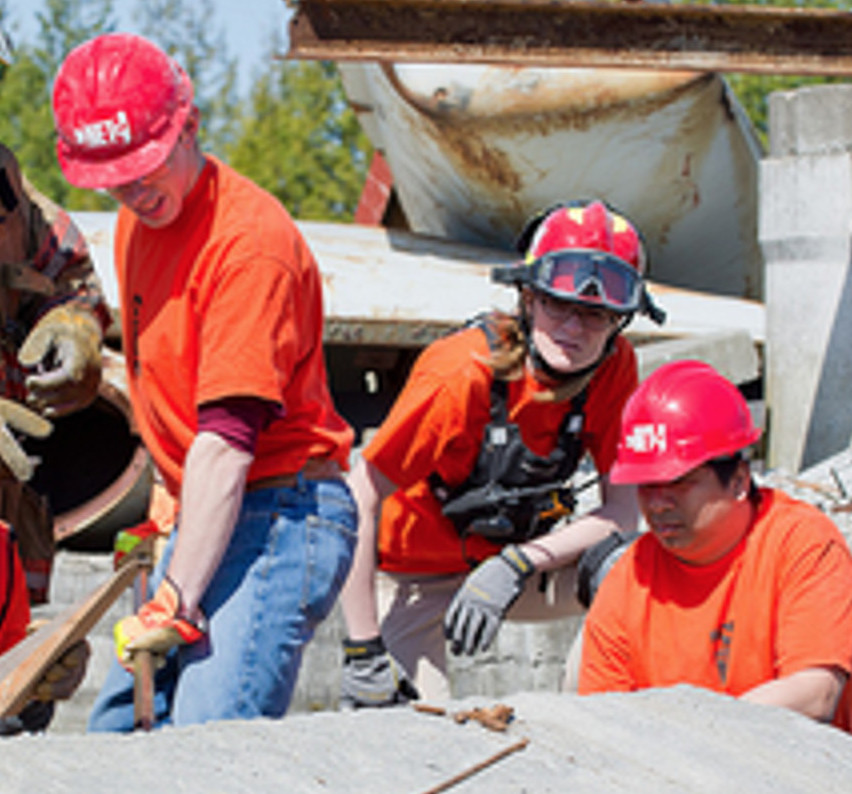
\includegraphics[scale=0.95]{graphics/PortlandNETs2.jpeg}}} % Image background; * means only on this page
\vspace*{6cm}     %from the top of page
\centering{
\normalfont\fontsize{35}{35}\sffamily\selectfont
\textbf{CERT Program Innovation: \\
Creative Options and Recommendations}\\  % Book title
\vspace*{7cm}    % between title and client/author lines
{\LARGE Produced for: \\
Portland Bureau of Emergency Management\\
\vspace*{1cm}   % between client and author
Produced by: \\
Bruce D. Marron \\}  % Author name
} 
\endgroup

%----------------------------------------------------------------------------------------
%	COPYRIGHT PAGE
%----------------------------------------------------------------------------------------

\newpage
~\vfill
\thispagestyle{empty}

\noindent Cover image, \copyright\ Portland NET, 2017\\ % Copyright notice
\noindent Chapter image, \copyright\ Los Angeles County Community Disaster Resilience, 2017\\ % Copyright notice
\noindent \textit{Published 12 December 2017} % Printing/edition date

%\noindent \textsc{Projet Janvier-Mars 2015, Université de Bourgogne}\\
%\noindent Ce projet a été encadré par Hervé CARDOT.\\ % License information



%----------------------------------------------------------------------------------------
%	TABLE OF CONTENTS
%----------------------------------------------------------------------------------------

\chapterimage{graphics/LAResilience.jpeg} % heading image

\pagestyle{empty} % No headers

\renewcommand\contentsname{Table of Contents}
\renewcommand{\bibname}{Bibliography}
\tableofcontents% Print the table of contents itself

%\cleardoublepage % Forces the first chapter to start on an odd page so it's on the right

\pagestyle{fancy} % Print headers again

%%%%%%%%%%%%%%%%%%%%%%%%%%%%%%%%%%%%%%%
%	CHAPTER 1
\chapterimage{graphics/LAResilience.jpeg} % Chapter heading image
\chapter{A Brief Historical Perspective}
%%%%%%%%%%%%%%%%%%%%%%%%%%%%%%%%%%%%%%%%%

The inauguration of present day Community Emergency Response Teams (CERTs) in the US typically dates to 1985 when, spurred by the Los Angeles Fire Department (LAFD), the city of Los Angeles sent representatives to Tokyo, Japan to observe a community-wide earthquake response drill \autocite{simpson_community_2001}. The LAFD concerns related to community emergency response were most likely generated by the September 19, 1985 earthquake in Mexico City in which hundreds of volunteers, lacking adequate training, perished along with thousands of others. \textcite{simpson_community_2001} points to an earlier beginning and suggests that CERT programs could be considered the progeny of the Civil Defense program, the Cold War era effort aimed at preparing citizens for disaster spawned by nuclear war. Certainly there are similarities in the two programs, but it is their differences which can provide insights into maintaining the viability of present day CERT programs. The first notable difference is in perceived threat: the Civil Defense program faded as the public's level of perceived threat of nuclear war diminished. In contrast, CERT programs continue to flourish as more real disaster challenges are recognized by more and more communities. Florida must take the credit for having the insight to move the Los Angeles earthquake-centered model to address local risk, in this case hurricanes. More important is the second difference. \textcite{simpson_community_2001} believes that Civil Defense programs lost traction because \enquote{they did not carry out neighborhood building activities}. The Civil Defense program ultimately failed to be inclusive and relevant.\\

\noindent There are two additional historically relevant events that have directly affected the development of CERT programs. The first is federal involvement. Beginning in 1993 the Federal Emergency Management Agency (FEMA) began offering \enquote{train-the-trainer} courses at the Emergency Management Institute (EMI) in Emmitsburg, Maryland. Since then FEMA has changed the nature of the CERT program by encouraging \enquote{disaster resilient communities} and providing institutionalization, validation, standardization, facilitation, and promotion \autocite{simpson_community_2001}. Early in the development of CERT programs, communities struggled not only for identity in terms of name and mission, but also for access to training guidelines and materials. Now, with some degree of federal sponsorship, there are readily available materials and local CERT programs can feel confident and legitimate in their mission and training. The second historically relevant event was Hurricane Andrew. In 1992 Hurricane Andrew struck Florida and it became clear that the assumption of a 72-hr official response time was wrong. CERT programs, including the Portland NET program, now prepare volunteers and communities to be self-reliant for at least two weeks. Community members that have internalized the reality of official response time following a major disaster are likely to recognize the real value in becoming a CERT volunteer.


%%%%%%%%%%%%%%%%%%%%%%%%%%%%%%%%%%%%%%%%%%%%%%%
\chapterimage{graphics/LAResilience.jpeg} % Chapter heading image
\chapter{A Brief Look at the Literature}
%%%%%%%%%%%%%%%%%%%%%%%%%%%%%%%%%%%%%%%%%%%%%%%

\section{Volunteerism}
%\vspace{1em}
Developing effective strategies for the recruitment and retention of volunteers requires a fundamental understanding of volunteer motivations and expectations. Understanding the motivations that create volunteers is the key to recruitment efforts; understanding the expectations that when fulfilled, keep volunteers coming back is the key to retention efforts. Volunteer motivation is a complex state space along the axes of humanitarianism and egoism. That is to say, that people volunteer for many reasons such as career development, personal enhancement, social responsibility, concern for society, and social enjoyment \autocite{shields_young_2009}. Ultimately, volunteers are motivated by both self-interest and altruism, often acting to reinforce each other. For example, \textcite{fahey_training_2002} note that the Volunteer Ambulance Corps of Tasmania program attracts people who are interested in \enquote*{learning new skills} as well as those who have the urge to \enquote*{assist the community.} There is some evidence that younger volunteers may be motivated more by financial and career success while older volunteers may be motivated by social responsibility \autocite{shields_young_2009}.



\section{Recruitment and Retention of Volunteers}
%\vspace{1em}

Recruitment efforts begin with organization evaluation. A program manager responsible for volunteer recruitment would be expected (1) to evaluate the organization's volunteer climate, (2) to detail the types of volunteer jobs that are needed and develop appropriate volunteer job descriptions, (3) to accurately  describe and characterize the organization's current volunteers, and (4) to understand the influences that affect people's decision to volunteer. Once this background work is completed a volunteer program manager may consider the development of different promotional appeals. For example, some authors suggest that recruitment efforts should target different age subgroups, presumably because these subgroups have different motivations. \textcite{shields_young_2009}, however, emphasizes that \enquote{maximum marketing efficiency} is to be gained by concurrently highlighting a broad spectrum of themes. These are the themes that relate directly to the primary reservoirs of volunteer inspiration: humanitarianism, social responsibility, and personal development.\\

\noindent Regardless of style, the central message in any recruitment appeal must be the importance of the organization's mission \autocite{wymer_jr._conceptual_2001}. Consistently, volunteers report that the main reasons for joining an organization (wanting to give to the
community, maintaining and expanding skills) must be deductively apparent in the organization's mission statement \autocite{ranse_engaging_2010}. Thus, a recruitment message should always have an explicit statement of mission and logical action links derived from the mission statement that support the main reasons for volunteering. \textcite{shields_young_2009} offers a simple but effective message scheme, which when adapted for the Portland NET program, would look something like,\\
\fbox{
\begin{minipage} [t][][c]{0.80\linewidth}

\includegraphics[scale=0.10]{graphics/PBEM_logo.jpg}
\textbf{Portland Bureau of Emergency Management}\\
\textit{Disaster risk reduction through leadership and coordination.}\\

Following a major disaster, first responders who provide fire and medical services will not be able to meet the demand for these services. Factors such as number of victims, communication failures and road blockages will prevent people from accessing emergency services that they have come to expect at a moment's notice through 911. People will have to rely on each other for help in order to meet their immediate life saving and life sustaining needs. \\


\includegraphics[scale=0.25]{graphics/NET_logo.jpg}
\textbf{Portland Neighborhood Emergency Team Program}\\
 When you volunteer for Portland NET ...\\
...you will actively participate in important activities that make a difference.\\
...you will have the opportunity to better yourself personally and professionally.\\
...you will make a difference in the lives of others.\\
...you will make connections with others.
 \end{minipage}
}

\bigskip
\bigskip
\noindent Volunteers remain with an organization when they experience high levels of connectedness, uniqueness, engagement, appreciation and empowerment \autocite{shields_young_2009}. High levels of connectedness result from being part of a group with which one shares goals, values, respect, and trust. Volunteers experience a feeling of uniqueness when they believe that they contribute a unique combination of talents and personality to the organization. Volunteers experience engagement when they have opportunities to demonstrate their skills, and they experience appreciation and personal empowerment when they are recognized as having made a real difference. Thus, retention efforts must focus on cultivating a volunteer's role identity. Perhaps surprisingly, researchers have discovered that training is a key element in cultivating and maintaining role identity. Both \textcite{ranse_engaging_2010} and \textcite{fahey_training_2002} report that training and related activities were by far the most frequently stated activities enjoyed by volunteers in emergency management organizations. These researchers advocate for training not only as a recruitment tool, but more importantly as a strong retention tool. Conversely, poorly delivered, irregular, and inflexible training can result in the loss of volunteers.


\vspace{2em}
\section{Some Notable CERT Programs}
%\vspace{1em}
Three CERT programs stand out for creating clever training opportunities and organizational innovations. The first is the Florida CERT Association, a 501(c)(3) (nonprofit) organization that supports statewide CERT training and education. Of note is that the Florida CERT Association has partnered with Universal Studios to create an annual mass casualty incident (MCI) drill at Universal Studios in Orlando, Florida (www.flacertassociation.org) . This amazing event includes pyrotechnics, overturned buses, wrecked airplanes, and hundreds of victims with moulage and makeup donated by Universal Studios. The event is open to all CERT teams and organizations throughout Florida.\\

\noindent The second noteworthy CERT program is the Area E Regional CERT, a regional organization in Los Angeles County, California. This regional organization is comprised of 25 member cities which are not incorporated by the City of Los Angeles (laareaecacert.samariteam.com). The Area E Regional CERT provides member cities with mutual aid support by way of training materials, CERT program managers, coordinators, instructors, and training mentors. The organization offers CERT trainings in Spanish, an annual training exercise for all member city CERT teams, and social events.  As an organizational innovation, the regional association promotes advanced CERT (ACERT) programs within each member city. The ACERT programs boast unique trainings: traffic control, crowd control, incident command support, monitored crime scene assistance, missing persons search, monitored evacuation assistance, and victim support services. The ACERT programs also have created specialized CERT teams, as for example, a response team that is prepared to deploy within the first 12 hours of an incident and a recovery team that is prepared to deploy as relief team. Both of these ACERT teams can convene within an hour for regional deployment and within 30 minutes for a local emergency. Perhaps unique to the Area E Regional CERT is the Red Cross CERT Fusion Academy, a joint training effort with the American Red Cross. \\

\noindent Finally, the Office of Emergency Management in Kansas City, Missouri has developed a variety of innovations targeting volunteer retention. Premier among these is the Kansas City CERT Rodeo, a friendly competition among the CERT teams volunteering in the eight county Kansas City metropolitan area (www.preparemetrokc.org). The rodeo event is masterfully designed to improve CERT program performance at the individual level, the team level, and the regional level. At the individual level CERT volunteers are required to demonstrate their skills in timed and graded exercises. At the team level CERT teams must mobilize, organize, and successfully realize a diverse set of disaster-scale challenge tasks. These tasks also are timed and graded. At the regional level there are timed and graded events that require cross-team cooperation. There also is plenty of built-in social mixing so that all the teams get to know one another and ideally, form professional relationships as well as individual friendships. The Kansas City Metropolitan Emergency Manager's Committee and the Kansas City Regional CERT developed the \textit{Rodeo in a Box} toolkit. The toolkit includes training videos and the introductory manual, \textit{CERT Rodeo in a Box: A Guide to Planning and Hosting Your Own CERT Rodeo}. Kansas City won an Honorable Mention in the category of Outstanding CERT Initiatives at the FEMA Individual and Community Preparedness Awards in 2014. Other Kansas City CERT innovations include Treasure Hunts, where two-way radio fundamentals are reinforced by teams communicating to solve the clues leading to a \enquote{treasure} of CERT supplies, and Wooden Bucks, a volunteer rewards program that allows volunteers to earn tokens for every four hours of participation in a class, a drill, or an actual incident where they provide assistance. The Wooden Bucks can be redeemed for CERT pack items like new light sticks, batteries, or replacement bandages.
 
\vspace{2em}
\section{The Concept of Community Resilience}
%\vspace{1em}
Resilience is a word that, like sustainability, has popular appeal but often is used without formal definition. This is not to say that formal definitions of resilience are unavailable. Rather, there are many useful definitions of resilience but they are system, context and scale dependent. Before examining how a definition of resilience could be appropriately applied to human communities under disaster, a brief review of various definitions of resilience is provided.\\

\noindent The concept of resilience is coupled with system disturbance. That is, resilience is concerned with a system's functionality and stability following a perturbation that is decidedly outside the normal range of intensity, extent, or duration. \textit{Engineering resilience} is often used to describe how quickly a physical (mechanical) system returns to a point of equilibrium \autocite{walker_resilience_2006}. More complicated, \textit{ecological resilience} recognizes that biological systems, as well as the social systems created by living beings, are complex adaptive systems. Complex adaptive systems have various stable states (basins of attraction) which are separated by thresholds. When a threshold is crossed the system may reorganize to a new regime with completely different functionalities. Thus ecological resilience tries to evaluate how much disturbance and change a system can endure before it shifts to a new basin. Engineering resilience is about the ability to \enquote {bounce back} while ecological resilience is about the ability to \enquote {get back at all.} Ecological resilience also is applied to social–ecological systems. \textcite {berkes_community_2013} define such resilience as \enquote{the capacity of the system to continually change and adapt and yet remain within critical thresholds. It may be formally defined as the capacity of a system to absorb disturbance and reorganize while undergoing change so as to still retain essentially the same function, structure, identity, and feedbacks.} \textit{Psychological resilience} is interested in how and why some individuals are better than others at coping with major disturbances in their lives. Here, resilience is seen as a continual process of personal development in building strengths to face adversity and create adaptation strategies rather than as a stable outcome to be reached and maintained \autocite{berkes_community_2013}. Like ecological resilience, the process is nonlinear.\\

\noindent The conceptual and applied development of \textit{community resilience} is relatively new. There are, therefore, various definitions of community resilience. \textcite{magis_community_2010} defines community resilience as \enquote{the existence, development, and engagement of community resources by community members to thrive in an environment characterized by change, uncertainty, unpredictability, and surprise. Members of resilient communities intentionally develop personal and collective capacity that they engage to respond to and influence change, to sustain and renew the community, and to develop new trajectories for the communities’ future. Community resilience is evidenced in the community’s successful response to crisis or opportunity or change, its successful implementation of plans, its development of new trajectories and futures for itself, and its adaptation to changes within and outside the community.} The Canadian Center for Community Renewal
defines a resilient community as \enquote{one that takes intentional action to enhance the personal and collective capacity of its citizens and institutions to respond to and influence the course of social and economic change.} \textcite{berkes_community_2013} suggest that at the core, community resilience is governed by agency and the capacity to self-organize. But there are apparently many factors that contribute to agency and self-organization such as people–place connections; values and beliefs; knowledge, skills and learning; social networks; engaged governance (involving collaborative institutions); a diverse and innovative economy; community infrastructure; leadership; and a positive outlook, including readiness to accept change. \textcite{magis_community_2010} lists another set of factors: community resources and their access; active agents; the ability for collective action; the ability for strategic action; equity; and impact.\\

\noindent Ultimately community resilience is about building social capital. It appears possible to create social capital through the agency of the community members themselves (through community challenges) as well as by external change agents that use well-known approaches in community development. These are programs that augment community strengths and community relationships. Community-specific CERT programs are likely to do just that. Table~\ref{tab:bm1} provides a typology for resilience. Figure~\ref{fig:bm1} shows the factors affecting the core of community resilience according to Berkes and Ross.\\


\begin{table}[!htbp]
  \caption{A typology of resilience (adapted from Berkes \& Ross, 2013).} 
  \label{tab:bm1} 
\begin{tabular}{ll}
\toprule
Resilience Typology &  Aspects \\
\midrule
Engineering & Fixed, single equilibrium state; resilient if system\\
            & returns rapidly to equilibrium \\
&  \\
Ecological & Complex adaptive systems; self-organizing; multiple stable states;\\
           & NOT in thermodynamic equilibrium; subject to constant disturbance;\\
           & resilient if system retains the same function, structure, identity, \\
           & and feedbacks after a disturbance\\
& \\
Psychological & Continual personal development processes; resilient if transcend \\
              & adversity, adapt to the environment, and maintain internal integration; \\
              & resilience builds with experience but can be overwhelmed if personal \\
              & tolerance thresholds are crossed\\
& \\
Community  & Continual community development processes of capacity building \\
           & and social learning; resilient if can manifest agency and \\
           & self-organization; resilience builds with experience but can be \\
           & overwhelmed with the loss of infrastructure and services\\
\bottomrule
\end{tabular}
\end{table} 


\begin{figure}
  \begin{center}
    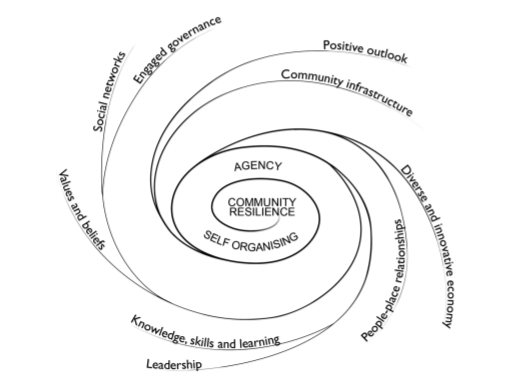
\includegraphics[scale=0.95]{graphics/Community_Resilience.jpeg}
    \caption{The factors that affect the core of community resilience (from Berkes \& Ross, 2013)}
    \label{fig:bm1}
  \end{center}
\end{figure}






%\vspace{1em}

%%%%%%%%%%%%%%%%%%%%%%%%%%%%%%%%%%%%%%%%%%%%%%%%%
\chapterimage{graphics/LAResilience.jpeg} % Chapter heading image
\chapter{Recommendations}
%%%%%%%%%%%%%%%%%%%%%%%%%%%%%%%%%%%%%%%%%%%%%%%%%%%%

\section{Structured Decision Making}
The resilience of any complex system is a function of its structure; specifically, the adaptability and robust nature of the relationships between its components. In social systems where an organizing framework is put in place to create a structure for the transfers of matter, energy, and information for a specific goal, some form of structured decision making is required if the social system is to have robust resilience. Structured decision making is simply a formal adaptive management mechanism that provides informational feedback as soon as possible after a change (decision) is made. Structured decision making is sequential, evidence-based decision making.  Structured decision making optimizes self-organization under change. That is, structured decision making provides the information needed to add, change, and evolve system structure.

\section{Recommendations}

The following list includes a variety of recommendations aimed at evolving the structure of the Portland NET program. These recommendations are strategies to increase volunteer diversity, retention, safety, and efficacy. The recommendations are made with the highest ethical intent and heart-felt purpose: to promote and safeguard community disaster preparedness and response in every single Portland neighborhood.\\

\begin{enumerate}
  \item \textbf{Create an iconic, Portland NET ambassador} -- To meet its diversity and community-level disaster preparedness goals, the Portland NET program must become an integral and highly visible part of the community landscape. An iconic Portland NET ambassador can make this happen. The Portland NET ambassador supports other worthy community service organizations (e.g., Immigrant and Refugee Community Organization, Native American and Youth and Family Center, Portland Mercado, etc.) by attending and volunteering at their events. In addition to the standard presentations at Office of Neighborhood Involvement-sanctioned neighborhood coalitions and neighborhood associations, the Portland NET ambassador creates opportunities, through personal connections, to make mini-presentations at tango festivals, at bluegrass workshops, at dragon boat practices, at the Portland Farmer's Market, and virtually anywhere people gather. Additionally, the Portland NET ambassador is a regular voice on local and community radio (KBOO, KMHD, KQAC) and creates news worthy events to be carried by local newspaper and television outlets. Real community outreach means being a caring and joyful friend to the community. \\
  \item \textbf{Create novel CERT teams} -- Drawing on inspiration from the Area E Regional CERT (see above), Portland NET could consider creating locally appropriate CERT teams. For example, how about bicycle-powered teams? Or river-based teams? The response and recovery types of teams created by Area E Regional CERT also could be considered.\\
  \item \textbf{Create novel training and productivity tools} -- Again and again researchers report that developed and delivered training is a retention tool for emergency management organizations \autocite{ranse_engaging_2010, fahey_training_2002}. Portland NET could follow the innovations championed by Kansas City such as the Kansas City CERT Rodeo, Treasure Hunts, and Wooden Bucks. And in addition to the delivered training why not begin to develop in-house training materials? Certainly small-scale video projects could be a start. These initial projects could highlight specific skill sets but could spark excitement for teams to script, shoot, and produce longer works. This is certainly doable with simple equipment and readily available video editing software (Linux \textit{AviDemux}, Mac \textit{iMovie}, Windows \textit{Movie Maker}). Another idea is to create one or more Portland NET phone applications (apps). Phone apps are increasingly used by researchers and are a huge success in citizen science organizations such as iNaturalist (www.inaturalist.org). Portland NET could develop volunteer-powered phone apps to help with (a) risk assessment in support of PBEM's accreditation by the Emergency Management Accreditation Program (EMAP). Note that EMAP certification requires that an Emergency Management Program has a Hazard Identification, Risk Assessment (HIRA) component that \enquote{identifies the natural and human-caused hazards that potentially impact the jurisdiction using multiple sources...[and] assesses the risk and vulnerability of people, property, the environment, and its own operations from these hazards}; (b) updating the Commodity Point of Distribution plan; (c) developing a plan to coordinate with the private sector during emergency response and recovery; and (d) activating the Damage Assessment Plan where residents and first responders could self-report losses.\\
  \item \textbf{Create regional and national connections} -- Portland NET could be the hub of a regional CERT organization. If, like the Florida CERT Association, such a regional association was a 501(c)(3) (nonprofit) organization, it would allow for independent grant funding opportunities to support regional CERT training and education. Clearly, the establishment of good relations with nearby CERT programs enhances disaster preparedness by boosting social capital. Similarly, Portland NET can reach out and make connections to other excellent CERT programs around the country to share ideas, challenges, and materials. It might even be possible to do some cross-training by sending our teams to advanced or unique training events and by inviting other teams to Portland for training events.\\
  \item \textbf{Create some appropriate climate of fun} -- Disasters are deadly serious. Disaster preparedness need not be. In fact, the success of disaster preparedness and recovery at the neighborhood level is predicated on social networks of trust and caring. Neighborhood resilience is built with social capital. CERT programs that are overly populated by what \textcite{karl_give_2008} term task-oriented volunteers (as opposed to people-oriented volunteers) probably suffer from the \enquote*{serious syndrome.} Without a social balancing force of fun, the serious syndrome can reduce overall real-world effectiveness because it depopulates diversity. Task-oriented volunteers view social interaction as an unnecessary distraction while volunteering; people-oriented volunteers need joyful and fun social interaction while volunteering. In a constantly serious environment people-oriented volunteers will experience reduced satisfaction leading to loss of volunteers. Thus, \textcite{karl_give_2008} notes that \enquote{managers of volunteers could expect positive outcomes from creating a fun work environment or implementing a culture of fun.} That said, caution must be exercised when implementing efforts at fun into the volunteer work environment: the task-oriented volunteers must be made to feel comfortable, too. If done without care, fun behaviors may be perceived as silly and frivolous activities that could insult those who feel they are volunteering for serious and honorable reasons. The goal is a balanced, diverse volunteer pool. Creating an appropriate climate of fun in the Portland NET community might start with simple eye-catching events. For example, in addition to a booth at Sunday Parkways events, why not have NET volunteers in full gear biking en masse to a boom box beat? What about staged rescue operations with moulaged victims at Last Thursday events? The basic idea here is to encourage dedicated NET volunteers to perform in a more relaxed and fun environment.
\end{enumerate}
  




% ----------------------------------------------------------------------------------------
% 	BIBLIOGRAPHY
% ----------------------------------------------------------------------------------------
          

\printbibliography



\end{document}
